\documentclass{article}
\usepackage{graphicx} % Required for inserting images
\usepackage{pgfplots}
\usepackage{adjustbox}
\usepackage{multicol}
\usepackage{float}
\usepackage{booktabs}

\title{DAE Project One}
\author{
Sayfullah Jumoorty (2430888)
\\ \\
Muhammed Muaaz Dawood (2425639)
\\ \\
Mujammil Mohsin Gulam Sakhidas (2436109)
}
\date{May 2024}

\begin{document}

\maketitle

\section*{Question 1}

a)  The model fits the data very well for both the training and the test data, with a $R^2$ score of 89.52\%  and 77.75\%  respectively. Figure \ref{CLMCTM} shows the scatter plot of CLM vs CTM.

\begin{figure}[H]
\centering
\includegraphics[width=0.6\textwidth]{CLM.png}
\caption{CLM vs CTM}
\label{CLMCTM}
\end{figure}
\noindent b)  The model fits the data poorly for both the training and the test data, with a $R^2$ score of 33.68\%  and 33.29\% respectively. Figure \ref{AGECTM} shows the scatter plot of AGE vs CTM.

\begin{figure}[H]
\centering
\includegraphics[width=0.6\textwidth]{AGE.png}
\caption{AGE vs CTM}
\label{AGECTM}
\end{figure}

\noindent c)  The model fits the data poorly for both the training and the test data, with a $R^2$ score of 26.20\%  and -11.09\% respectively. Figure \ref{LVLCTM} shows the scatter plot of LVL vs CTM.

\begin{figure}[H]
\centering
\includegraphics[width=0.6\textwidth]{LVL.png}
\caption{LVL vs CTM}
\label{LVLCTM}
\end{figure}

\noindent d)  The model fits the data poorly for both the training and the test data, with a $R^2$ score of 29.03\%  and 18.40\% respectively. Figure \ref{SDYCTM} shows the scatter plot of SDY vs CTM.

\begin{figure}[H]
\centering
\includegraphics[width=0.6\textwidth]{SDY.png}
\caption{SDY vs CTM}
\label{SDYCTM}
\end{figure}

\section*{Question 2}
We aim to predict CTM using the variables AGE, CLM, LVL, and SDY. Our goal is to observe a strong correlation between CTM and these independent variables. The correlation matrix can be seen in Figure \ref{CM}.

\begin{figure}[H]
\centering
\includegraphics[width=0.6\textwidth]{Correlation.png}
\caption{Correlation Matrix}
\label{CM}
\end{figure}


\noindent Upon analysis, we find that CLM exhibits the highest correlation with CTM, followed by AGE, SDY, and LVL. It is essential to ensure a minimal correlation between the independent variables:
\begin{multicols}{2} % 
\begin{itemize}
  \item AGE: Highly correlated with CLM and LVL, while exhibiting a low correlation with SDY.
  \item CLM: Shows a high correlation with AGE and SDY, and a low correlation with LVL.
  \item LVL: Exhibits a high correlation with AGE and a low correlation with both CLM and SDY.
  \item SDY: Highly correlated with CLM and weakly correlated with AGE and LVL.
\end{itemize}
\end{multicols}

\noindent While this analysis provides valuable insights, further testing is necessary to determine which features to retain and which to discard. For this purpose, we employ the Adjusted \(R^2\) metric:

\begin{enumerate}
  \item Base model (CLM only) Adjusted \(R^2\): 0.878.
  \item Model with CLM and AGE Adjusted \(R^2\): 0.878.
  \item Model with CLM, AGE, and LVL Adjusted \(R^2\): 0.879.
  \item Model with CLM, AGE, LVL, and SDY Adjusted \(R^2\): 0.882.
\end{enumerate}  


\noindent Initially, we employed the base model using CLM to predict CTM, given its highest correlation. Subsequently, we iteratively included other features to observe their impact on the Adjusted \(R^2\) score. The addition of AGE did not affect the score, while the inclusion of LVL increased it by 0.001. Finally, incorporating SDY raised the score by 0.002.
\\\\
Consequently, only LVL and SDY demonstrated a positive effect on the model. Since AGE had no impact on the Adjusted \(R^2\) score, we proceed to evaluate the model's performance with and without AGE as a predictor. We iterate through different model configurations to make comparisons:

\begin{itemize}
  \item The model featuring 'CLM', 'SDY', and 'LVL' as features performs optimally with an MSE of 2.19.
  \item Conversely, the model incorporating 'CLM', 'SDY', 'LVL', and 'AGE' as features yields an MSE of 2.26.
\end{itemize}

\noindent The plot of errors can be seen in Figure \ref{RP} and \ref{RPAGE}.

\begin{figure}[H]
\centering
\includegraphics[width=0.6\textwidth]{RP without age.png}
\caption{Residual Plot for CLM, SDY, and LVL}
\label{RP}
\end{figure}

\begin{figure}[H]
\centering
\includegraphics[width=0.6\textwidth]{RP with age .png}
\caption{Residual Plot for CLM, SDY, LVL and AGE}
\label{RPAGE}
\end{figure}

\section*{Question 3}
The MSE analysis clearly demonstrates that Model 1, featuring 'CLM', 'SDY', and 'LVL' as its predictors, outperforms Model 2, which additionally incorporates the 'AGE' feature. This outcome suggests that 'AGE' doesn't contribute significantly to predicting the client's trust measure ('CTM'), potentially due to its high correlation with other features, as indicated by the correlation matrix provided.
\\\\
Given the notably higher correlation between 'AGE' and other features compared to its correlation with 'CTM', it's reasonable to expect that 'AGE' might not offer much unique predictive power for 'CTM' when already considering features like 'CLM', 'SDY', and 'LVL'. Hence, its inclusion leads to diminished predictive performance, as observed in the higher MSE for Model 2.
\\\\
While the difference in MSE between the two models is slight, the superior performance of Model 1 underscores its suitability for predicting 'CTM'.

\section*{Question 4}
To re-iterate, the problem at hand is to predict the number of cases a lawyer will handle in a given month (\textbf{CTM}) based on the number of cases they handled the previous month (\textbf{CLM}), their age (\textbf{AGE}), their level of seniority within the firm (\textbf{LVL}), and the number of sick days they took in the last year (\textbf{SDY}).
\\\\
\noindent The final model chosen is the one that includes \textbf{CLM}, \textbf{SDY}, and \textbf{LVL} as predictor variables. This model makes sense for the following reasons:

\begin{enumerate}
    \item \textbf{CLM (Cases Last Month)}: The number of cases a lawyer handled in the previous month is likely to be a strong predictor of the number of cases they will handle in the current month. There is often a continuity in the workload of lawyers, and their past performance can be a good indicator of their current performance.
    
    \item \textbf{SDY (Sick Days in the Last Year)}: The number of sick days taken by a lawyer in the previous year can impact their productivity and, consequently, the number of cases they handle. If a lawyer has been frequently absent due to illness, it can lead to a lower case load or a backlog of work that needs to be cleared.
    
    \item \textbf{LVL (Level of Seniority)}: The level of seniority within the firm can influence the complexity and volume of cases assigned to a lawyer. Senior partners and managing partners are typically assigned more high-profile and complex cases, which may result in a higher case load compared to junior associates.
\end{enumerate}

\noindent The exclusion of \textbf{AGE} as a predictor variable makes sense because the analysis showed that it did not significantly improve the model's performance. While age could potentially be a factor in some cases (e.g., experience, energy levels), it does not seem to have a strong direct impact on the number of cases handled in this particular dataset.
\\\\
\noindent Additionally, the linear regression model assumes a linear relationship between the predictor variables and the target variable (\textbf{CTM}). This assumption seems reasonable for the chosen predictors, as they are likely to have a relatively linear effect on the number of cases handled by a lawyer.
\\\\
\noindent However, it is important to note that the linear regression model may not capture potential non-linear relationships or interactions between the predictor variables. If such relationships exist, more complex models or feature engineering techniques may be required to improve the model's performance.
\\\\
\noindent Furthermore, the model's assumptions, such as the independence of observations and the normality of residuals, should be checked to ensure the validity of the linear regression approach.
\\\\
\noindent Overall, the chosen model, which includes \textbf{CLM}, \textbf{SDY}, and \textbf{LVL} as predictor variables, appears to be a reasonable choice based on the given information and the context of the problem. It incorporates relevant factors that are expected to influence a lawyer's case load while excluding variables that did not significantly improve the model's performance.

\section*{Question 5}

\subsection*{Scatter Plots:}

\begin{figure}[H]
    \centering
    \includegraphics[width=1.1\textwidth]{ScatterPlots.png}
    \caption{Scatter Plots}
    \label{ScatterPlots}
\end{figure}

The scatter plots provided in Figure \ref*{ScatterPlots} show a visual representation of the relationships between the predictor variables (\textbf{CLM}, \textbf{SDY}, and \textbf{LVL}) and the target variable (\textbf{CTM}). From the plots, we can observe the following:

\begin{enumerate}
    \item \textbf{CLM vs. CTM}: There appears to be a strong positive linear relationship between the number of cases last month (\textbf{CLM}) and the number of cases this month (\textbf{CTM}). As \textbf{CLM} increases, \textbf{CTM} tends to increase as well, which aligns with the intuition that a lawyer's workload is often consistent from one month to the next.
    
    \item \textbf{SDY vs. CTM}: The scatter plot shows a slight negative relationship between the number of sick days taken in the last year (\textbf{SDY}) and the number of cases this month (\textbf{CTM}). This relationship makes sense, as lawyers who have taken more sick days may have had less time to work on cases, potentially leading to a lower case load.
    
    \item \textbf{LVL vs. CTM}: The scatter plot suggests a positive relationship between the lawyer's level of seniority (\textbf{LVL}) and the number of cases this month (\textbf{CTM}). Higher levels of seniority, such as senior partners or managing partners, are generally assigned more complex and high-profile cases, which could explain the higher case loads.
\end{enumerate}

\noindent Overall, the scatter plots provide visual support for including these predictor variables in the model, as they exhibit relationships with the target variable that align with our intuition and understanding of the problem domain.

\subsection*{Residual Plot:}

\begin{figure}[H]
    \centering
    \includegraphics[width=0.6\textwidth]{ResidualPlot.png}
    \caption{Residual Plot}
    \label{ResidualPlot}
\end{figure}

The residual plot in Figure \ref*{ResidualPlot} displays the differences between the predicted values and the actual values (residuals) against the predicted values. In an ideal linear regression model, the residuals should be randomly distributed around the horizontal line ($y=0$), with no apparent patterns or trends.
\\\\
From the residual plot, we can observe that the residuals are approximately evenly distributed around the horizontal line, with no clear patterns or trends. This suggests that the assumptions of the linear regression model, such as the assumption of homoscedasticity (constant variance of residuals) and the absence of patterns in the residuals, are reasonably met.
\\\\
However, it's worth noting that there are a few points with relatively large residuals, which may indicate potential outliers or data points that the model struggles to fit accurately.

\subsection*{AIC and BIC:}

The Akaike Information Criterion (AIC) and Bayesian Information Criterion (BIC) are metrics used to compare the relative quality of different models, with lower values indicating a better fit while considering model complexity.

For the provided output:
\begin{itemize}
    \item AIC: 703.60
    \item BIC: 716.80
\end{itemize}

\noindent These values can be compared with alternative models or used to assess the impact of adding or removing predictor variables. Lower AIC and BIC values generally indicate a better-fitting model, but the interpretation also depends on the specific context and the magnitude of the differences between models.

\subsection*{Multicollinearity Check (VIF):}

The Variance Inflation Factor (VIF) measures the degree of multicollinearity, which occurs when predictor variables are highly correlated with each other. High VIF values (typically above 5 or 10) indicate potential multicollinearity issues, which can affect the reliability of the model's coefficients and their interpretability.
\\\\
From the provided output:

\begin{table}[H]
  \centering
  \caption{Multicollinearity check (VIF)}
    \begin{tabular}{ccc}
    \toprule
    \textbf{VIF Factor} & \textbf{Features} \\
    \midrule
    4.428688 & const \\
    1.739526 & CLM \\
    1.398538 & SDY \\
    1.292021 & LVL \\
    \bottomrule
    \end{tabular}%
  \label{tab:vif}%
\end{table}%

\noindent We can observe that the VIF value for the constant term is relatively high (4.428688), which is expected and not a cause for concern. The VIF values for the predictor variables \textbf{CLM} (1.739526), \textbf{SDY} (1.398538), and \textbf{LVL} (1.292021) are all below the commonly used threshold of 5, indicating that multicollinearity is not a significant issue in this model.
\\\\
However, it's worth noting that the VIF value for \textbf{CLM} (1.739526) is slightly higher than the others, suggesting a moderate level of correlation between \textbf{CLM} and the other predictor variables. While this does not necessarily invalidate the model, it's something to be aware of and potentially investigate further if necessary.
\\\\
Overall, the provided heuristics and visualizations support the chosen model by demonstrating the relationships between the predictor variables and the target variable, assessing the model's assumptions, and checking for potential issues such as multicollinearity.

\section*{Question 6}

The Table \ref{ENGFEATURES} contains the features that were engineered, Table \ref{COMBO} shows the models containing the different combinations of these features that we tested and their $R^2$ values can be seen in Figure \ref{R2BAR}.

\begin{table}[H]
\centering
\small
\begin{minipage}{0.45\textwidth}
    \centering
    \begin{adjustbox}{max width=\textwidth}
    \begin{tabular}{|l|}
    \hline
    \textbf{Engineered Features} \\
    \hline
    CLM\_squared \\
    CLM\_log \\
    SDY\_log \\
    CLM\_SDY\_interaction \\
    CLM\_mean \\
    CLM\_std \\
    SDY\_mean \\
    SDY\_std \\
    CLM\_ratio \\
    SDY\_ratio \\
    \hline
    \end{tabular}
    \end{adjustbox}
    \caption{List of engineered features}
    \label{ENGFEATURES}
\end{minipage}
\hfill
\begin{minipage}{0.45\textwidth}
    \centering
    \begin{adjustbox}{max width=\textwidth}
    \begin{tabular}{|l|l|}
    \hline
    \textbf{Model} & \textbf{Features} \\
    \hline
    Baseline & CLM SDY LVL \\
    \hline
    Model 1 & CLM SDY LVL CLM\_squared \\
    \hline
    Model 2 & CLM SDY LVL CLM\_log \\
    \hline
    Model 3 & CLM SDY LVL SDY\_log \\
    \hline
    Model 4 & CLM SDY LVL CLM\_SDY\_interaction \\
    \hline
    Model 5 & CLM SDY LVL CLM\_squared CLM\_log SDY\_log \\
            & CLM\_SDY\_interaction \\
    \hline
    Model 6 & CLM SDY LVL CLM\_squared CLM\_log SDY\_log \\
            & CLM\_SDY\_interaction CLM\_mean CLM\_std \\
    \hline
    Model 7 & CLM SDY LVL CLM\_squared CLM\_log SDY\_log \\
            & CLM\_SDY\_interaction SDY\_mean SDY\_std \\
    \hline
    Model 8 & CLM SDY LVL CLM\_squared CLM\_log SDY\_log \\
            & CLM\_SDY\_interaction CLM\_ratio SDY\_ratio \\
    \hline
    Model 9 & CLM SDY LVL CLM\_squared CLM\_log SDY\_log \\
            & CLM\_SDY\_interaction CLM\_mean CLM\_std \\
            & SDY\_mean SDY\_std CLM\_ratio SDY\_ratio \\
    \hline
    Model 10 & CLM SDY LVL CLM\_squared CLM\_log SDY\_log \\
             & CLM\_SDY\_interaction CLM\_mean CLM\_std \\
             & SDY\_mean SDY\_std CLM\_ratio SDY\_ratio \\
    \hline
    \end{tabular}
    \end{adjustbox}
    \caption{Combinations of the different engineered features}
    \label{COMBO}
\end{minipage}
\end{table}

\begin{figure}[H]
    \centering
    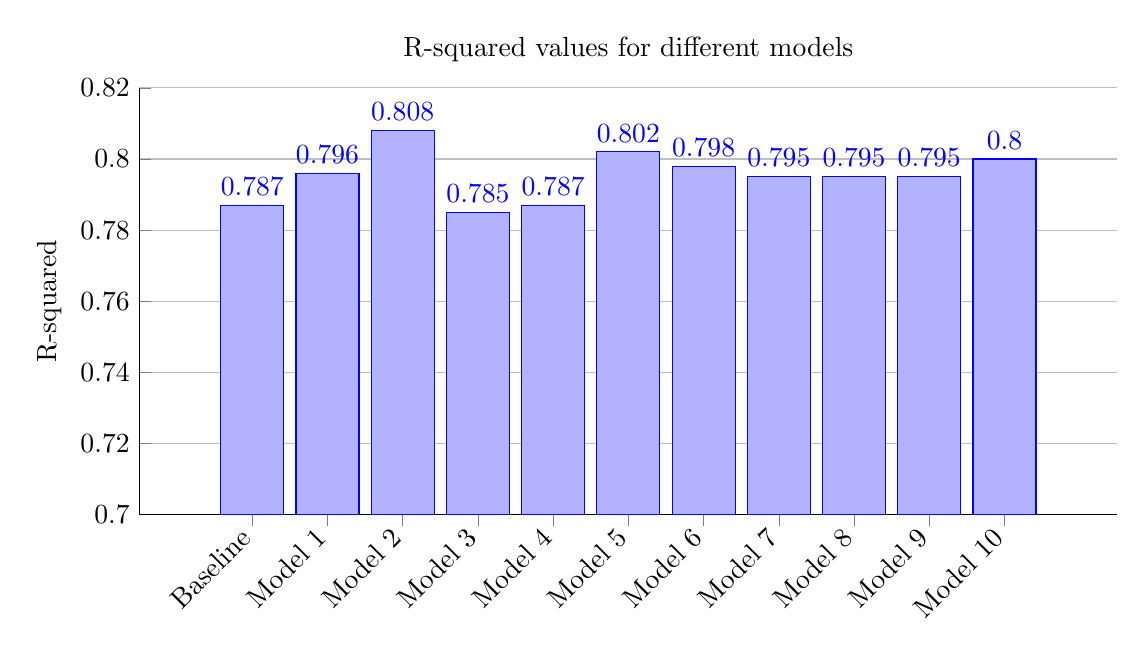
\begin{tikzpicture}
        \begin{axis}[
            ybar,
            xtick=data,
            nodes near coords={
                \pgfmathprintnumber[precision=3]{\pgfplotspointmeta}
            },
            nodes near coords align={vertical},
            ymin=0.7,
            ymax=0.82,
            ylabel={R-squared},
            xlabel={},
            width=14cm,
            height=7cm,
            enlarge x limits=0.15,
            bar width=8mm,
            axis lines*=left,
            ymajorgrids=true,
            xticklabel style={rotate=45,anchor=east},
            xticklabels={Baseline, Model 1, Model 2, Model 3, Model 4, Model 5, Model 6, Model 7, Model 8, Model 9, Model 10},
            legend style={at={(0.5,-0.2)},
                anchor=north,legend columns=-1},
            title={R-squared values for different models}
            ]
            \addplot coordinates {(0,0.787) (1,0.796) (2,0.808) (3,0.785) (4,0.787) (5,0.802) (6,0.798) (7,0.795) (8,0.795) (9,0.795) (10,0.800)};
        \end{axis}
    \end{tikzpicture}
    \caption{R-squared values for different models}
    \label{R2BAR}
\end{figure}



\noindent The engineered features that have been included in the models are reasonable choices and can potentially improve the model's performance in predicting the number of cases a lawyer will handle this month (CTM). Here's a discussion of the rationale behind these engineered features:

\begin{enumerate}
    \item \textbf{Polynomial Features}:
    \begin{itemize}
        \item \texttt{CLM\_squared}: Including the squared term of the number of cases a lawyer handled last month (CLM) can capture potential non-linear relationships between CLM and CTM. This feature allows the model to account for situations where the effect of CLM on CTM may not be strictly linear.
    \end{itemize}
    
    \item \textbf{Logarithmic Transformations}:
    \begin{itemize}
        \item \texttt{CLM\_log}: Taking the logarithm of CLM can help model scenarios where the relationship between CLM and CTM may follow an exponential or logarithmic pattern.
        \item \texttt{SDY\_log}: Similarly, the logarithmic transformation of the number of sick days taken in the last year (SDY) can capture non-linear relationships between SDY and CTM.
    \end{itemize}
    
    \item \textbf{Interaction Terms}:
    \begin{itemize}
        \item \texttt{CLM\_SDY\_interaction}: This feature represents the interaction between CLM and SDY. It allows the model to account for potential combined effects of these two variables on CTM. For example, the impact of sick days on the case load may depend on the number of cases handled in the previous month.
    \end{itemize}
    
    \item \textbf{Group-based Features}:
    \begin{itemize}
        \item \texttt{CLM\_mean}, \texttt{CLM\_std}, \texttt{SDY\_mean}, \texttt{SDY\_std}: These features capture the mean and standard deviation of CLM and SDY within each level of seniority (LVL). They can help the model account for potential differences in the case load distributions across different seniority levels.
    \end{itemize}
    
    \item \textbf{Ratio Features}:
    \begin{itemize}
        \item \texttt{CLM\_ratio}, \texttt{SDY\_ratio}: These features represent the ratio of a lawyer's CLM and SDY to the sum of CLM and SDY within their seniority level, respectively. These features can capture the relative workload and absenteeism of a lawyer compared to their peers at the same seniority level.
    \end{itemize}
\end{enumerate}

\section*{Question 7}
Among the models presented in the solution, Model 2 stands out as the best-performing model, with the highest R-squared value of 0.808. Let's examine why the combination of features in Model 2 makes sense for predicting the number of cases a lawyer will handle in a given month (CTM).
\\\\
Model 2 includes the following features:
\begin{itemize}
    \item CLM: The number of cases the lawyer handled last month
    \item SDY: The number of sick days the lawyer took in the last year
    \item LVL: The lawyer's level of seniority within the firm
    \item CLM\_log: The logarithmic transformation of CLM
\end{itemize}

\noindent The inclusion of the original predictor variables (CLM, SDY, LVL) in Model 2 is logical and aligns with domain knowledge. CLM reflects the lawyer's recent workload and productivity, which is likely to be a strong predictor of their current month's case load. SDY can impact a lawyer's availability and efficiency, potentially affecting their case load. LVL is relevant as it may determine the complexity and volume of cases assigned to a lawyer based on their seniority.
\\\\
The addition of the logarithmic transformation of CLM (CLM\_log) in Model 2 is a meaningful engineered feature. It captures the non-linear relationship between CLM and CTM, accounting for the potential diminishing impact of an increase in the previous month's case load on the current month's case load as CLM grows larger. The logarithmic transformation compresses the scale of CLM, giving more importance to relative changes rather than absolute changes.
\\\\
Model 2 strikes a balance between capturing important relationships and maintaining simplicity. By including only one engineered feature (CLM\_log) alongside the original predictor variables, the model remains relatively easy to interpret and explain. The logarithmic transformation is a straightforward mathematical operation, making it accessible to stakeholders without extensive technical expertise.
\\\\
The improvement in Model 2's performance compared to the baseline model, as indicated by the higher R-squared value, supports the appropriateness of this feature combination. The inclusion of CLM\_log captures additional information that helps explain the variability in CTM, leading to a better fit of the model to the data.
\\\\
In conclusion, the combination of features in Model 2 makes sense for predicting CTM. It incorporates relevant predictor variables that align with domain knowledge and adds a meaningful engineered feature that captures the non-linear relationship between CLM and CTM. The model maintains simplicity and makes it easy to interpret while demonstrating improved performance.

\end{document}
